\section{Demo Proposal}
\label{sec:scenarios}

\begin{figure*}[ht]
\center
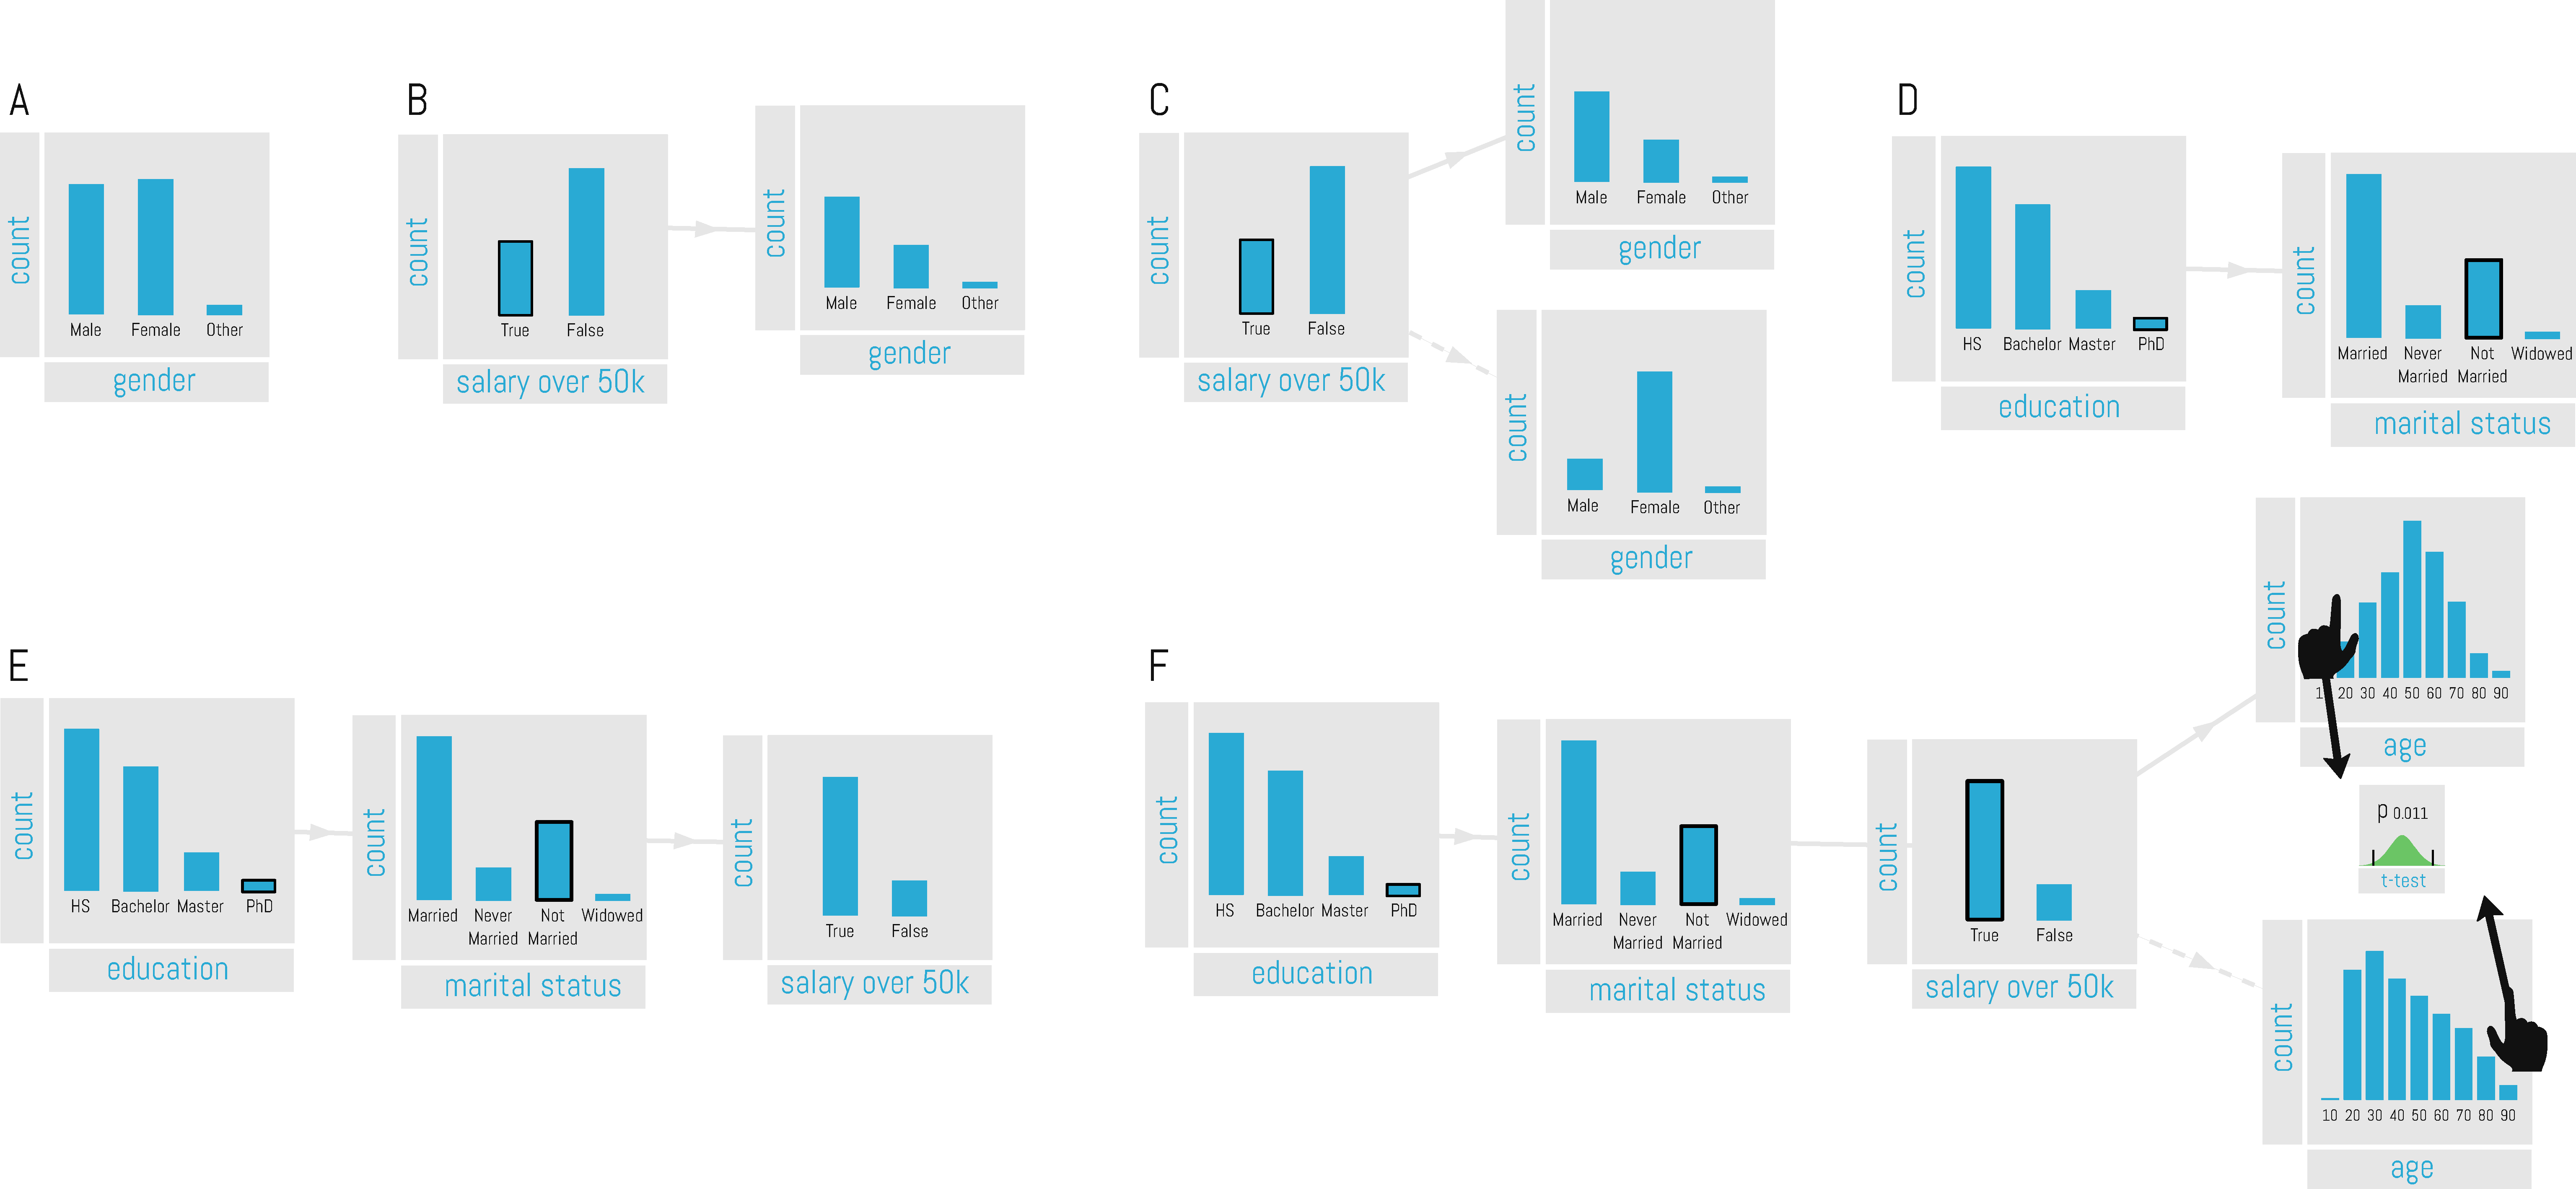
\includegraphics[width=\textwidth]{figures/storyboard.pdf}
\caption{Storyboard showing a user exploring a dataset through \system{}.}
\label{fig:sb}
\vspace{-4ex}
\end{figure*}

To demonstrate \system{}, we use various publicly available datasets and a dataset obtained via a survey on Amazon Mechanical Turk~\cite{binnig2017sustainable}. This survey collected answers to 69 questions from 104 participants. Questions cover a wide range of habits and opinions and are mostly unrelated conceptually, such as ``Do you believe in aliens?'',  ``What is your eye color?'' and ``How tall are you?''. 

Figure \ref{fig:sb} shows an example storyboard of a user exploring the aforementioned survey dataset through \system{}. A user, Eve, starts out by looking at two attributes she is interested in: age and height (A top). She wants to see if there is a correlation between the two and thus creates a third visualization where she plots them against each other (A bottom). Just from visual inspection, age and height do not seem to be correlated. However, Eve wants to be sure and thus explicitly creates a hypothesis test. She uses a multitouch gesture (dragging the two visualization close to each other) and \system{} automatically picks and computes an appropriate test (a correlation test in this case) (B). This confirms Eve's intuition that the two attributes are not correlated. Eve continues to look at the answers to the question ``Do you know what SQL is?''. It looks like a bit more than half the people answered this question with yes (C left). Our user wants to find out what other attributes are good predictors if someone knows SQL. Her first hunch is to look at age. She creates a query that allows her to filter the SQL attribute by people who are over 50 years old. For this age group the y-axis ordering of the two bars switched: less people in this age group know of SQL (C right). Visually it seems that this is quite a big effect, however \system{} automatically executed a hypothesis test for this comparison that tells Eve this is in fact not statistically significant (C, red block on the right-hand side). Eve goes on to do a similar query. This time checking if people who know who Mike Stonebraker is have a higher chance of knowing SQL. The hypothesis test automatically computed by \system{} reinforces what Eve sees: this is a significant effect. 

Eve realizes this manual exploration is becoming fairly laborious and decides to continue by using the automatic visualization recommender that \system{} provides. By tapping on the SQL attribute visualization she gets a handle to invoke a search for recommendation visualization. The handle shows that she has 70\% of exploration budget left (E). The visualisation recommendation system works through touch gestures. Dragging away from the handle invokes it, whereby the angle and the length of the drag-path determine the amount of exploration budget that should be spent and if \system{} should look for similar or dissimilar visualization (+ and - signs on the handle) (F and G). Eve chooses to spend 20\% of her budget and to look for dissimilar visualizations (G). \system{} progressively computes and ranks recommendations until the allotted budget is used up and presents thumbnails of results (H). Eve can press-and-hold on thumbnails to preview the result. Overlaid in purple she sees that people who know programming have a higher chance of also knowing SQL (I). She wants to see more detail about that relation and drags the thumbnail out which in turn creates a filter chain similar to the one she created manually before. 

All hypothesis test results are automatically tracked and subject to multiple hypothesis correction by \system{} and displayed in a scrollable list through which Eve can, at any time, inspect and obtain additional information about any hypothesis (Figure \ref{fig:ui}). 
